\documentclass[11pt]{article}
\usepackage[utf8]{inputenc}
\usepackage[russian]{babel}

\title{\textbf{Теоретическая Неорганическая Химия}\\ {\normalsize (3 модуль)}}
\author{1 курс ФХ HИУ ВШЭ}
\date{23 октября 2019}
\usepackage{graphicx}
\begin{document}
\begin{titlepage}
\maketitle
\end{titlepage}
\tableofcontents

\section*{Квантовые числа} 
\begin{itemize}
\item Главное $n$ - энергия электрона в атоме. $[1,2,3,\ldots]$

\item Побочное, орбитлаьное, азимутальное - $l, m_l$ - "форма орбитали", форма изоповерхности волновой функции, "угловая составляющая" волновой функции(углы в полярной системе координат)$[0,1,2\ldots n-1]$

\item Магнитное - $m_l, m_s, m$ - определяет ориентацию волновой функции(орбитали) относительно вектора напряженности внешнего магнитного поля. $[-l \ldots 0\ldots l]$

\item Спиновое - "направление вращения" или направление полета электрона$[-\frac 12;\frac 12]$

\end{itemize}


\section*{Изменение электронных оболочек атомов}




\subsubsection*{Правило Клечковского}

Заполнение происходит в порядке возрастания суммы квантовых чисел $n+l$

Основное и возбужденное состояния - соответственно состояния с наименьшей энергией, и все другие состояния. При переходе из возбужденного состояния в основное выделяется энергия, например в виде излучения. Возможен и обратный вариант.

Это широко используется для анализа и изучения вещества - единственный недеструктивный метод изучения.

В пределах одного уровня орбитали неодинаковы по энергии. Различие по энергии между уровнями и подуровнями тем ниже, чем выше эти (под)уровни ($\Delta(2s-3s)>\Delta(3s-4s)$)

Спаренные электроны невыгодны по двум причинам - закон Кулона против сближения двух отрицательно заряженных частиц, и энергия, затрачиваемая на изменение спина.

Спин можно считать моментом импульса электрона, так как его движение наиболее близко к вращательному.

Изучать состояния электронов можно по частотам излучения и соответствующим переходам.
\subsection*{Экранирование электронов}
Орбитали "заслоняются" нижележащими орбиталями, энергия этого состояния повысится, связь электрона с ядром ослабевает, и т.д.

Эффективный заряд ядра - считается по правилу Слейтера. Эффективный заряд для, например, $3s NA$ - около 2.5. Приводит это к тому, что электрон от него оторвать несложно.

$$E_{eff} = Z - S$$

$S$ - константа экранирования.
Считаем ее так:
\begin{itemize}
\item Пишем конфигурацию
(1s) (2s, 2p) (3s, 3p) (3d) (4s, 4p) (4d) (4f) (5s, 5p) (5d)…
Расположите электроны согласно правилу Клечковского.
\item Любые электроны, расположенные справа от интересующего вас электрона, не оказывают влияния на константу экранирования.
\item Константа экранирования для каждой группы рассчитывается как сумма следующих составляющих:
\item Все остальные электроны, находящиеся в одной группе с интересующим нас электроном, экранируют 0,35 единиц заряда ядра. Исключение составляет 1s-группа, где один электрон считается только за 0,30.
\item В случая группы, относящейся к [s, p] типу, берут 0,85 единиц на каждый электрон (n-1) оболочки и 1,00 единицу на каждый электрон (n-2) и следующих оболочек.
\item В случая группы, относящейся к [d] или [f] типу, берут 1,00 единицу на каждый электрон, находящийся слева от этой орбитали.
\end{itemize}

Из-за проникающей способности возникает много чего интересного, например, влияние ядра на $5s$ больше чем на $4d$.

Все эти закономерности приводят по сути к периодическому закону, открытому Менделеевым за четыре десятка лет до появления вот этого физического обоснования.

\subsection*{Периодичность изменения свойств элементов}
Свойства:
\begin{itemize}
\item Атомный и ионный радиусы - проблемные величины, так как есть правило неопределенности. Определить радиус нельзя, но можно определить радиус участка, в котором вероятность нахождения электрона равна 0.9 или 0.8 или чему-то еще
\item Энергия ионизации и сродства к электрону

Кстати, энергия ионизации всегда положительна, а вот сродство к электрону может иметь любой знак

Энергия ионизации - это энергия орбитали!

\item Электроотрицательность
\end{itemize}

По периоду вправо энергия ионизации растет, ЭО тоже растет из-за увеличения заряда ядра и заряда оболочки, при том что число оболочек не меняется.

По группе вниз энергия ионизации и ЭО падают, так как становится больше оболочек. 

Правда, у энергии ионизации есть немонотонность, в отличие от всех остальных характеристик, меняется менее линейно. Так, ЩМ из-за хорошей проникающей способности $s$-орбитали, в отличие от инертных газов, слабо меняют энергию ионизации по группе.

Сродство к электрону - энергия, выделяемая или поглощаемая при присоединении электрона. По группе вниз падает, по периоду вправо растет, но это тренды в целом, а так все немонотонно и зависит от устойчивости получаемой частицы.

Так, ЩЗМ принимают электроны сильно менее охотно, чем ЩМ, так как ЩМ принимает электрон на тот подуровень, что уже начал заполняться, а ЩЗМ - на новый, более высокий по энергии.

Электроотрицательность - веичина синтетическая, считается по разным формулам, отражает способность оттягивать электроны на себя.
\begin{itemize}
\item Поллинг
$$\chi = k*(\left(X-Y\right)_meas - \left(X-Y\right)_expected)$$
\item Малликен
$$\chi = \frac 12 \left(|F| + |I|\right)$$
\item Олред-Рохов
$$\chi = k\frac{Z_eff}{r^2} + c$$
\end{itemize}
Все три модели дают схожие цифры, так что использовать можно любую. Константы $k$ и $c$ - используют для "подгона" друг к другу.

\section*{Свойства ионных соединений}

\begin{itemize}
\item Нельзя обнаружить свойства атома в ионе
\item Свойства катиона и аниона независимы
\item 
\end{itemize}

\subsection*{Ионные соеднения в газовой фазе}

$NaCl$ - только в ионной плазме. Там одни ионы, соединения уже нет.

$LiCl$ - существует в газовой фазе в виде пар. Существует ли там чисто ионная связь? Сравним с моделью - протоном и электроном на расстоянии 1 ангстрем. Сравнивать будем дипольное взаимодействие.

Дипольный момент равен $D = 1 \varepsilon A^0$. Сравнение с фторидом лития дает 92\% ионности и 8\% ковалентности для последнего. Для сравнения, у воды ионность порядка 33\%.

Свойтва в твердой фазе

\begin{itemize}
\item Твердые, хрупкие
\item Непластичные
\item Бесконечная периодическая структура
\end{itemize}

Решетки могут иметь разную форму. Например, $NaCl$ и $CsCl$ имеют разные решетки - гцк и оцк соответственно.
TODO вставить картинуи решеток.

Соотношение атомов в ячейке надо считать осторожно, учитывая \textbf{во сколько ячеек входит каждый атом}!

Координационные числа должны быть одинаковы для $AB$, отличаются вдвое для $AB_2$ - ну, иначе не сойдется.

Решетка зависит от соотношения размеров катиона-аниона. Для $r^+/r^- = [1, 1.37]$ - характерна решетка $CsCl$, для $[1.37..2.44]$ - $CsCl$, для большего - $ZnS$.

\subsection*{Модель жестких сфер}

Чтобы было можно говорить о радиусах, считаем их жесткими сферами, несжимаемыми. Катионы в среднем имеют меньший радиус чем анионы.

Из предположения о жесткости следует наличие предела сжатия, равного размеру "шариков".
$$E = \frac{Z_1Z_2e^2}{4\pi\varepsilon_0d_0}$$

$e$ - заряд электрона, соответственно $Z_1, Z_2$ в относительных единицах.

Ясно, что на графике энергии есть ассимптота, равная сумме радиусов.

\subsection*{Периодичность изменения ионных радиусов}

По группе вниз - растет, из-за появления новых электронных обоолочек. У переходных элементов - какая-то немонотонная хрень, поговорим о ней в след. модуле.

\textbf{Координационное число} - число противоионов, окружающих ион

У октаэдра КЧ=6, у куба - 8. Но от КЧ должен зависеть радиус. Да, экспериментально так и есть. Определяют РСА и решением системы линейных уравнений(РСА дает расстояние между ионами, взяв 4 таких, решаем уравнения и получаем радиусы).

Расстояние между атомами в газе меньше. Почему? Из-за КЧ - взаимодействие с одним соседей в $n$ раз сильнее чем с каждым из $n$.

Энергия кристаллической решетки состоит из двух компонентов - энергия взаимодействия и энергия отталкивания. Как и любая сумма возрастающего и убывающего компонентов, такая конструкция имеет экстремум. Этот экстремум - точка с координатами $(R_1+R_2;E)$.

Энергия решетки выражается формулой:
$$E = \frac{Z_1Z_2E^2N_AA}{4\pi \varepsilon_0R}(1-\frac 1n) $$
где $N_a$ - константа Авогадро,\\
$A$ - постоянная Маделунга,\\
$n$ - показатель сжимаемости иона,\\
$R$ - расстояние между ионами.

Постоянная Маделунга зависит от типа решетки, и растет от роста КЧ.

Практически энергию решетки определяют с помощью \textbf{цикла Борна-Габера} - цикла Гесса, включающего энергетические эффекты ионизации аниона и катиона, испарения, и т.д.
\begin{figure}[htp]
\centering
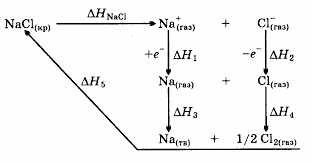
\includegraphics[scale=1.00]{born-gaber.png}
\caption{}
\label{}
\end{figure}

\subsection*{Отклонения от модели жестких сфер}
\begin{itemize}
\item Деформация оболочек ионов при больших радиусах - поляризация ионов.

Приводит к различным эффектам, вроде уголковой формы молекул вида $AB_2$ в газовой фазе, характерной для галогенидов бария и частично стронция.
\item Контакт одноименно заряженых ионов - отклонения от типичных свойств ионного соединения.

Например, у иодида лития расстояние между ионами больше суммы ионных радиусов из-за отталкивания иодид-ионов.
\end{itemize}

\subsection*{Ионные соединения в растворе}

Разрушение кристаллической решетки компенсируется энергией сольватациии, то есть взаимодействия растворителя с растворенным веществом. Это сотни-тысячи кДж/моль.
В растворе ионного соединения есть
\begin{itemize}
\item Сольватированные ионы сами по себе
\item Ионные пары:
\begin{itemize}
\item контактные:
$$(solv)A^+|B^-(solv)$$
\item сольватно-разделенные
$$(solv)A^+|solv|B^-(solv)$$
\end{itemize}
\end{itemize}

\subsection*{Необычные ионные соединения}

ЩМ в жидком аммиаке.

ЩМ+криптанды - $[Cs(18-crown-6)_2]e$, $[Na^+(18-crown-6)_2]Na^-$ - проводят ток.
\section*{Ковалентные соединения}

Леменовский Дмитрий Анатольевич

Определение хим. связи - отсутствует. В основе описания связи - закон Кулона, который, кстати, эмпирический.

Молекулярные соединения - связи внутри молекул много сильнее, чем между ними. 

Ковалентные связи выделяют по следующим признакам:
\begin{itemize}
\item обособленность связи

\item наличие длинны

\item определенные углы
\end{itemize}

Ковалентный радиус - табличная величина. Определяют или делением на 2 расстояния между ядрами в случае симметричной связи, или решением системы уравнений. Некая ошибка будет всегда, так как есть тепловой разброс длинны связи. Плюс при наличии заместителей все тоже меняется. Так, с $CCl_4$ расстояние $C-Cl$ равно 1.76 ангстрем, а в $O_2N-CCl_3$ - 1.65 ангстрем

Для водорода, однако, все не как у всех. Соединение $H_2$ - имеет радиус 0.37, а во всех других соединениях типа углеводородов - 0.30. Поэтому в справочниках не пишут 0.37.

Рассмотрим радиусы элементов $IVa$ группы:
\begin{center}
\begin{tabular}{|l|l|l|l|}
\hline
	$C$ & $Si$ & $Ge$ & $Sn$\\
\hline
	0.77 & 1.17 & 1.22 & 1.40\\
\hline
\end{tabular}

\begin{tabular}{|l|l|l|l|}
\hline
	$N$ & $P$ & $As$ & $Sb$\\
\hline
	0.70 & 1.10 & 1.21 & 1.41\\
\hline
\end{tabular}

\begin{tabular}{|l|l|l|l|}
\hline
	$O$ & $S$ & $Se$ & $Te$\\
\hline
	0.66 & 1.04 & 1.17 & 1.37\\
\hline
\end{tabular}

\begin{tabular}{|l|l|l|l|}
\hline
	$F$ & $Cl$ & $Br$ & $I$\\
\hline
	0.64 & 0.99 & 1.14 & 1.33\\
\hline
\end{tabular}
\end{center}

Настоящей квантовой химии не будет, но чуть-чуть вводить что-то придется. 
\subsection*{Методы описания связей}
Два метода описания химической связи, используемые сейчас - \textbf{метод валентных связей} и \textbf{метод молекулярных орбиталей}.
В первом связь представляется как результат спаривания электронов и перекрывания электронных оболочек. Проблема в нем сразу в постулате - образование электронной пары - невыгодный энергетически процесс. Плюс проблемы с правилом инертного газа - половину молекул вроде $HNO_3$ или того почему $O_2$ - бирадикал нормально не объясняет.

В какой-то степени исправляет эту ситуацию метод молекулярных орбиталей. Там вводится понятие волновой функции. Надо учитывать геометрию, так как в атоме самом по себе никаких осей нет, а оси и геометрия появляются при появлении взаимодействий.

По методу молекулярных орбиталей, есть лишь одна молекулярная орбиталь вместо всех атомных орбиталей. Упрощения этой модели: 
\begin{itemize}
\item разделение волновых функций атомного ядра и электронов
\item разделение электронов на валентные и невалентные
\item разделение электронов валентного уровня по связям и атомам
\end{itemize}

На примере молекулы $H_2$($r=0.74$ ангстрем, $E = -458 \frac{kJ}{mol}$):
\begin{figure}[htp]
\centering
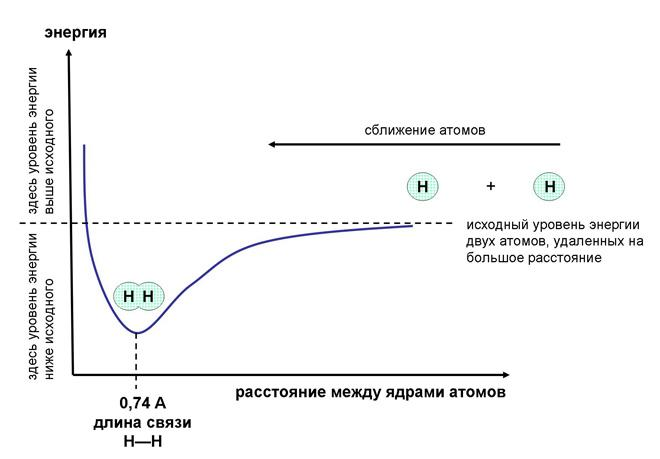
\includegraphics[scale=2.00]{h2-er.png}
\caption{}
\label{}
\end{figure}
Для атомов водорода есть волновые функции их электронов $\psi_1$ и $\psi_2$, кроме того, есть волновая функция всей молекулы $$\psi_{H_2} = \psi_1 + \psi_2$$. Рассчетом по уравнению Шредингера получим $r=0.94$ ангстрем и энергией $24 \frac{kJ}{mol}$. С точностью все, конечно, плохо,но хоть молекула получидась, уже что-то

Можно добавить функции с обменяными электронами.
$$\psi_{H_2} = \psi_{A_2}*\psi_{B_1} + \psi_{A_1}*\psi_{B_2} $$
 Это добавит точности, мы получим уже $r=0.82$ ангстрем $303 \frac{kJ}{mol}$

Можно добавить еще и функции, где все электроны на одном атоме, и т.д \ldots Энергия, понятно, чтанет все ближе и ближе к экспериментам(график внизу).

Кстати, как раз делокализация электронов и есть причина образования связи, она-то, в отличие от спаривания, выгодна энергетически.

Попробуем теперь нарисовать какие-нибудь картинки. Энергия в атоме квантована, то есть электрон и его энергию можно сравнить с "лесенкой",  а не с наклонной плоскостью.

Если сложить две оболочки в фазе, получим "горбик" - если в фазе, или ноь - если в противофазе. Это и есть процесс образования связи. На самом деле, двухжлектронная связь не двухэлектронная, так как из этих двух электронов большая часть находится у ядра..





\end{document}










